\documentclass{report}
\usepackage{mathtools}
\usepackage{amsmath}
\usepackage{amssymb}
\usepackage{amsfonts}
\usepackage{graphicx}
\usepackage{float}
\usepackage{multirow}
\usepackage{verbatim}

\linespread{1.3}
\setlength{\parindent}{0em}
\setlength{\parskip}{1em}
\setcounter{secnumdepth}{0}
\setcounter{MaxMatrixCols}{20}
\renewcommand{\arraystretch}{1.5}

\newcommand{\ts}{\textsuperscript}
\newcommand{\diff}{\mathop{}\!\mathrm{d}}
\newcommand{\prob}{\mathbb{P}}
\newcommand{\expect}{\mathbb{E}}
\newcommand{\var}{\text{Var}}

\DeclarePairedDelimiter{\abs}{\lvert}{\rvert}
\DeclarePairedDelimiter\norm{\lVert}{\rVert}
\DeclarePairedDelimiter\p{\lparan}{\rparan}

\title{COMS3000 notes}
\author{Joshua Hwang (44302650)}

\begin{document}
\maketitle
\tableofcontents
\chapter*{Prerequisite maths}
We must recall how to calculate the extended Euler's algorithm and discrete
logarithms.

Should be noted for the discrete logarithm to exist,
\begin{align*}
    \log_a (c) \mod n \\
\end{align*}

$n$ must be prime and $a$ needs to be a generator.

I will assume you know how to calculate the extended Euler's algorithm.

\chapter{Information security}
\section{Basic terms}
This first chapter will talk about definitions.

There are three things we can do with risk; accept it, transfer it (insurance)
or reduce it (control it).

Information security is all about protective measures and dealing with potential
damages. Some of these protective measures include; prevantative measures,
detective measures (to know when, how and who caused damage) and reactive
measures (allows us to recover from damages).

The information security can be categorised into the CIA triad.
\begin{description}
    \item [Confidentiality] Prevent unauthorised disclosure of information
    \item [Integrity] Prevent unauthorised modification of information
    \item [Availability] Prevent unauthorised witholding of information i.e. DoS
\end{description}

We can extend these first three aspects with two more
\begin{description}
    \item [Authenticity] Make sure the author/sender is as claimed
    \item [Non-repudiation] People can't escape contracts by claiming that it
        was a forgery.
\end{description}

Being trusted and trustworthy are two separate ideas.
Hopefully the difference is obvious.
Direct trust can be developed by two parties.
Indirect trust involves trusting a third party who claims others are trustworthy.
Trust will be explored later on.

\section{Risk management}
Risk management is the process concerned with identification, measurements,
controls and minimisation of security risks in information systems to a level
appropriate to what the asset is worth.

The following definitions are quite dry and dense so be prepared.

Risk management helps determine and optimise for the appropriate cost/benefit
for protective measures.

Identify, measure, control and minimise or eliminate attacks.
This is done through: risk assessment, cost benefit analysis, selection,
implementation and evaluation of security features and countermeasures and
an overall security review.

The definition of risk as determined by ISO/IEC 27000:2018 is,
`\textbf{effect of uncertainty of objectives}'.
Where an objective is a result to be achieved. (e.g\. our data gets locked up)

The definition of threat as determined by ISO/IEC 27000:2018 is,
`\textbf{potential cause of an unwanted incident,
which can result in harm to a system
or organization}' (e.g.\ the rival company may want to perform underhanded
corporate tactics)

The definition of vulnerability as determined by ISO/IEC 27000:2018 is,
`\textbf{weakness of an asset or control that can be exploited by one or more
threats}' (e.g.\ system is exposed to the internet and could run random
binaries from the internet)

The definition of risk assessment as determined by ISO/IEC 27000:2018 is,
`\textbf{overall process of risk identification, risk analysis and risk
evaluation}`.

\section{Risk analysis}
A qunatitative risk analysis largely resolves around the following.
A model for quantifying the cost is taking the expected value of the
event occuring $prob \times impact$.

\begin{description}
    \item [ARO (Annualised Rate of Occurrence)] Number of times a year.

    \item [SLE (Single Loss Expectancy)]
        The impact of a single type of this event occurring.

    \item [ALE (Annualised Loss Expectancy)]
\end{description}

The equation is simple and is as follows,
\begin{align*}
    ALE &= ARO \times SLE
\end{align*}

It is often difficult however to get these probabilities and also to
quantify the impact and cost of an event.

Instead we might use a more qualitative method.
Risk assessment matrices.

\begin{figure}[h]
    \centering
    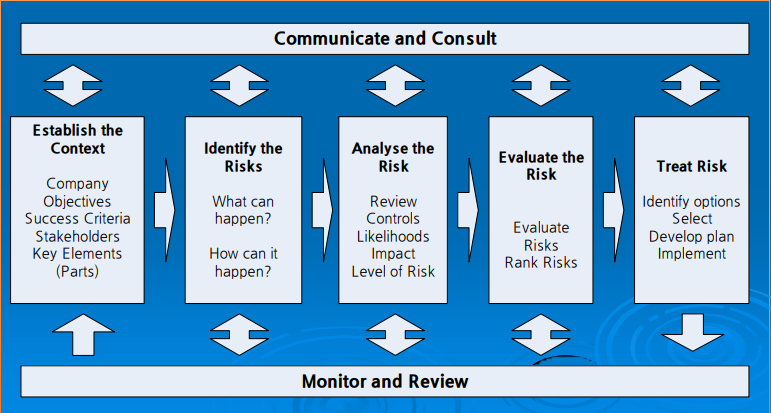
\includegraphics[width=\textwidth]{images/standards-flow.png}
    \caption{ISO31000:2018 Risk Management Principles and Guidelines}
\end{figure}

\chapter{Access Control}
There are two separate but important functions to establish identity:
\begin{description}
    \item [Identification] Determine who the entity is
    \item [Authentication] Verity and prove you are who you say you are.
\end{description}

Authorisation, once identity is established a decision can be made about
granting or denying access.

Most access control is determined by identity. Which has a second benefit of
accountability (we can track who did what when in the system).

\section{Authentication}
Passwords have been the goto for years. It is based on `something you know'.
There are many of problems incluing; forgetting the password, same password for
multiple places, weak passwords, passwords not kept in secret and not changing
default passwords.

Carna botnet was an attempt to scan and attempt default passwords on anything
connected to the internet. It obtained $\approx 500,000$
devices through Telnet mostly embedded systems in 2012.

Passwords can be guessed via bruteforce, socially engineered and tricked out of
humans, eavesdropped and keylogged. Many also store passwords in various places
like password managers which increases risk.

\chapter{Cryptography}
\begin{description}
    \item [Cryptography] is about keeping messages secure. It literally means
secret writing.

    \item [Cyrptanalysis] is the science of breaking message security.

    \item [Cryptology] is the theory associated with
        cryptography and cryptanalysis.
\end{description}

The aim of cryptography is confidentiality but it can also be used to
authenticate a user, ensure no messages have been modified and
might even be used for digital signing.

\section{Types of attacks}
Much like in MATH3302 we have the different types of cipher attacks:
\begin{description}
    \item [Ciphertext only]
        The attacker has obtained a piece of ciphertext but no decoding
    \item [Known-plaintext attack]
        The attacker has obtained a piece of ciphertext and its corresponding
        plaintext
    \item [Chosen-plaintext attack]
        The attacker has temporary access to the encryption machine
    \item [Adaptive Chosen-Plaintext attack]
        The attacker has the encryption machine for quite some time
\end{description}

\textbf{Side Channel Attacks} are attacks against an implementation rather than
the algorithm itself. We gain new information like, timing, power consumption
etc.

\section{Hash functions}
Hash functions compress an arbitrarily long input $x$ into a fixed size output.
They should be designed to be easy to compute.

One-way hash functions have the one-way property. It is computationally
infeasable to find $x$ given $h(x)$.
One-way is also called \textbf{pre-image resistance}.

Now cryptographic one-way functions have another property called
\textbf{collision resistance}.

An ideal one-way cryptographic function can be visualised as such.
`Has this input arrived before?' If yes re-return the output. If no, then
make a random sequence for this new input.
This model is called a \textbf{random oracle model}.

\textbf{Strong collision resistance} means its hard to find two distinct
$x_1$ and $x_2$ such that $h(x_1) = h(x_2)$
\textbf{Weak collision resistance (aka 2nd pre-image resistance)}
given a specific
$y=h(x_1)$ it is hard to find $x_2$ such that $h(x_1) = h(x_2)$

To find a weak collision we need $2^n$ but for a strong collision we just need
$2^{n/2}$ since birthday paradox.

A cryptographic hash is considered broken if collisions can be found with
significantly less work than brute force.

An offline attack on passwords is when the attacker has access to the hashes
of the password. The hacker can then apply numerous exploits on the file
to get a collision/reverse the hash.

\section{Cryptography keys}
The problem with using a different and hidden protocol for all communications
between people is that no one can talk to new people. Instead we have
cryptography keys which alter the algorithm in a way that still ensures it's
impractical to crack. This is \textbf{Kerckhoff's Principle},
`\textit{The security of a cipher should rely on the secrecy of the key only.}'

Computational security is measured by, the resources and time necessary for the
attacker to crack the cipher (with the key length we're using)
vs how long the information needs to be kept
secret.

\chapter{Types of ciphers}
As we learnt in MATH3302 there is no way yet to practically measure the security
of a cipher. It's either `too hard' to wrap our heads around or it's founded on
a computational problem that does not have efficient algorithms (yet).
Thus the goal of creating a cipher is computation security,
this is where the best
attack option is brute-force; there are no shortcuts to get to the key.
From here it's purely key length that determines security; it's a simple brute
force job.
The only way we can `prove' this is to show that our cipher is secure against
all currently known attacks.

\section{Old ciphers}
You should have seen and remembered many of these ciphers from MATH3302.

Caeser cipher where each letter is offset by a constant amount (this shift is
the key).

Monoalphabetic substitution cipher where the alphabet is shuffled randomly.

Vigenère cipher is an extension of the Caesar cipher where a secret set of
offsets (usually a word) is periodically used on the plaintext.

One time pads where we extend the Vigenère cipher so the secret word is the
length of the message. The secrete key doesn't get repeated. One time pads
are perfectly secure.

Transposition cipher where we create a matrix of the message (secret rows and
columns) we then read off the matrix in the transpose way.
\begin{figure}[h]
    \centering
    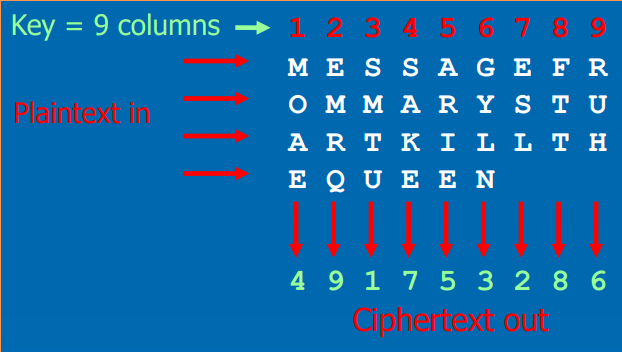
\includegraphics[width=\textwidth]{images/transpositioncipher.png}
\end{figure}

\section{Symmetric ciphers}
Many modern ciphers are product ciphers.
A product cipher is a composition of either substitutions or permutations
(which are also just substitutions). They are iterated several times to increase
security.

Feistel ciphers are what you've already seen in MATH3302 so I hope you remember
them. Many product ciphers are Feistel ciphers.

Transposition involving swapping the two blocks being encrypted.
Substitution using S-boxes.
Decryption is also encryption but with the round keys in reverse order.

Note that the F function does not have to be reversible since XOR twice results
in the original solution.

\subsection{Block ciphers}
\subsubsection{DES}
DES uses 16 rounds with 64 bit blocks and 56-bit key with 8 bits for parity.
The round function expands 32 bits into 48 bits.
The S-box converts 6 bits into 4 bits

The DES challenge was an attempt to break the DES by bruteforce.
\begin{description}
    \item [1997] took 3 months
    \item [1998] took 3 days and cost \$250K
    \item [1999] took 22 hours with machine created from the 1997 and 1998 challenges
    \item [2006] took 7 days for \$10K (COPACOBANA)
\end{description}

Each new key bit doubles the time required for a brute force. This means a
128-bit key will take 90 billion billion years for COPACOBANA to crack it.

Choosing to double DES via
\begin{align*}
    c &= E_{K2}(E_{K1}(p)) \\
    p &= D_{K1}(D_{K2}(c))
\end{align*}

Now we should theoretically have double the key size. Unfortunately 2-DES is
vulnerable to meet-in-the-middle attacks.

If you manage to find the inbetween value (so $E_{K1}(p) = D_{K2}(c)$) then we
can look for a collision between the two key spaces.
Because we need $x$ this is technically a known-plaintext attack.

Instead we use triple DES\@.
\begin{align*}
    c &= E(D(E(p)))
\end{align*}

You may not that we're decrypting for the second function this is so that if
$K1=K2=K3$ then this is essentially single DES\@. Which helps with compatibility.

\subsubsection{AES}
In 1998 NIST (US National Institue of Standards and Technology) announced
development of AES\@. In 2000 NIST chose the cipher we know as AES\@.

Selection process for AES was public and 15 candidates were brought;
5 were found to be broken,
5 weren't that good,
5 were finalists.
\begin{itemize}
    \item Serpent
    \item Rijndael
    \item Twofish
    \item Mars (IBM)
    \item RC6 (RSA Data Security Inc.)
\end{itemize}

Rijndael won with its symmetric block cipher (not Feistel).
128-bit data blocks
You could choose key lengths with 128 (10 rounds), 192 (12 rounds)
and 256 bytes (14 rounds). It could even be
extended though this feature is not part of the standard.

AES is seen as a block of data (an actual square).
\begin{enumerate}
    \item Initial round
    \item Adds the round key via XOR
    \item Normal rounds
        \begin{enumerate}
            \item Each byte is substituted via a lookup table.
            \item Each row is then shifted cyclically.
            \item The columns are mixed
            \item Add the round key like the initial round
        \end{enumerate}
    \item Final round. Same as Normal rounds but without mixing rows.
\end{enumerate}

The choice of S-box was based on a bunch of stuff that won't be covered.

The US Government uses
AES-128 is used for SECRET classification and
AES-192 or AES-256 for TOP SECRET\@.

Interestingly Intel and AMD have inbuilt AES instructions.

\subsubsection{Block cipher modes}
\textbf{ECB (electronic book mode)}
This involves generating a single key and XORing this key to each block of
input. This is obviously weak since we're using the same key for mutliple
plaintext and there is not dependency between the blocks.

The ECB mode is simple, implementation, parallelisable,
errors only affect that single block (blocks aren't dependent) but it is weak.
Replay attacks are possible. If the block sizes are small enough we could
potentially build a table of dictionary attacks for a block cipher.

\textbf{CBC}, \textbf{CFB} and \textbf{OFB} build off of ECB by embedding
dependency and feedback.

\textbf{CBC (cipher block chaining mode)} uses a single key but now the
encrypted block is XORed with the next message
block before being XORed with the key. The first block is XORed with an
initialisation vector (IV). Decryption involves XORing the key then XORing the
IV (in that order). CBC cannot be parallelised since each block is dependent on
the previous one.

Turns out IV does not need to be secret but it should be changed frequently.

CBC can actually self-recover from bit errors. [ZZZ I have no idea how or why]
This property could be used to determine the
differences caused by changes in bits.
CBC is the most commonly used cipher mode but may soon be overtaken by Counter
Mode.

\textbf{CFB (cipher feedback mode)} is very similar to CBC\@.
We start with an initial
vector and encrypt it. We take this encrypted vector and XOR the message onto
it; this is our first cipher block. We take this cipher block and use this as
our new initial vector which we encrypt and XOR the message onto.

We can extend the CFB by introducing an arbitrary $k$ bit shift after getting
the
new intial vector. We introduce this $k$ shift so we can get rid of error bits.
By shifting $k$ bits in an $n$ sized block we can get rid of the error after
$n/k + 1$ repeats ($n/k$ block and the initial block that started it).

CFB can actually recover from a whole block of the cipher getting deleted.
[ZZZ no idea how again]

\textbf{OFB (output feedback mode)} provides a slight modification of CFB\@.
In OFB we take
our intial vector and encrypt it. We then take this encrypted block and use it
as the next initial vector. After this we take the same encrypted vector and XOR
it to the message. Note in this model each following message is not
dependent on the previous one. Only the number of times the initial key was
encrypted.

Obviously if an error occurs in the setup then it won't propogate to the other
messages because the messages are independent of previous message blocks.

This method also allows us to optimise via precomputing the key and encryptions.
This method cannot recover from the loss of an entire ciphertext block however.

\textbf{CTR (counter mode)} we use a completely different approach.
We generate a nonce
and a counter. After every round we will bump up the counter and either XOR,
concatenate or add it to the nonce (if the nonce isn't random then we must only
use concatenation). We pass these nonce+counters into our encryptor and then
XOR or message onto the encrypted part.

Much like in the OFB the ciphers aren't dependent on each other but simply
dependent on the counter size. This means that errors aren't propogated.

\subsection{Side Channel Attacks}
AES implementations have been broken using Side Channel Attacks.
One implementation uses caches which makes certain inputs faster than usual.
You could probably use this information to attack the system.

\section{Stream Ciphers}
As you should already know block ciphers take blocks of the input and converts
it into blocks of encrypted input.
A stream cipher generates a stream of pseudorandom keys (unlike OTP which uses
truly random key stream)

Encryption usually involves XORing the pseudorandom keys.

\textbf{RC4} (aka Ron's Code who is also the R in RSA) is the most widely used
stream cipher, implemented in MS Word, Excel, Wireless LANs (WEP).

RC4 has been found to have some vulnerabilities.

\textbf{Lamport's Hashed Password Scheme}. Here
the idea is the create a sequence of one-time passwords using a one-way hash
function.

The client selects an initial secret password $p_0$
We can compute the $p_n = h(p_{n-1})$.
The server is keeping a track of the current $p$ and current $n$.
The server sends the client the current counter.
User sends $p_n$ and the server checks its own version with what was sent.
Now the server \textit{decrements} $n$ by one.
This way that if eavesdropping occurs
that the entire sequence doesn't get destroyed.

% Stopped at line 403

\end{document}
